\hypertarget{page_dyn_sys_sec_dyn_sys_intro}{}\subsection{Introduction}\label{page_dyn_sys_sec_dyn_sys_intro}
Let a {\itshape state} be a vector of real numbers. A dynamical system consists of such a state and a rule that describes how this state will change over time; it describes what future state follows from the current state. A typical example is radioactive decay, where the state $x$ is the number of atoms, and the rate of decay is $\frac{dx}{dt}$ proportional to $x$\+: $ \frac{dx}{dt} = -\alpha x$. Here, $\alpha$ is the `decay constant' and $\dot{x}$ is a shorthand for $\frac{dx}{dt}$. Such an evolution rule describes an implicit relation between the current state $ x(t) $ and the state a short time in the future $x(t+dt)$.

If we know the initial state of a dynamical system, e.\+g. $x_0\equiv x(0)=4$, we may compute the evolution of the state over time through {\itshape numerical} {\itshape integration}. This means we take the initial state $ x_0$, and iteratively compute subsequent states $x(t+dt)$ by computing the rate of change $\dot{x}$, and integrating this over the small time interval $dt$. A pseudo-\/code example is shown below for $x_0\equiv x(0)=4$, $dt=0.01s$ and $\alpha=6$.


\begin{DoxyCode}
alpha=6; \textcolor{comment}{// Decay constant}
dt=0.01; \textcolor{comment}{// Duration of one integration step}
x=4.0;   \textcolor{comment}{// Initial state}
t=0.0;   \textcolor{comment}{// Initial time}
\textcolor{keywordflow}{while} (t<1.5) \{
  dx = -alpha*x;  \textcolor{comment}{// Dynamical system rule}
  x = x + dx*dt;  \textcolor{comment}{// Project x into the future for a small time step dt (Euler integration)}
  t = t + dt;     \textcolor{comment}{// The future is now!}
\}
\end{DoxyCode}


This procedure is called ``integrating the system'', and leads the trajectory plotted below (shown for both $\alpha=6$ and $\alpha=3$.


\begin{DoxyImage}
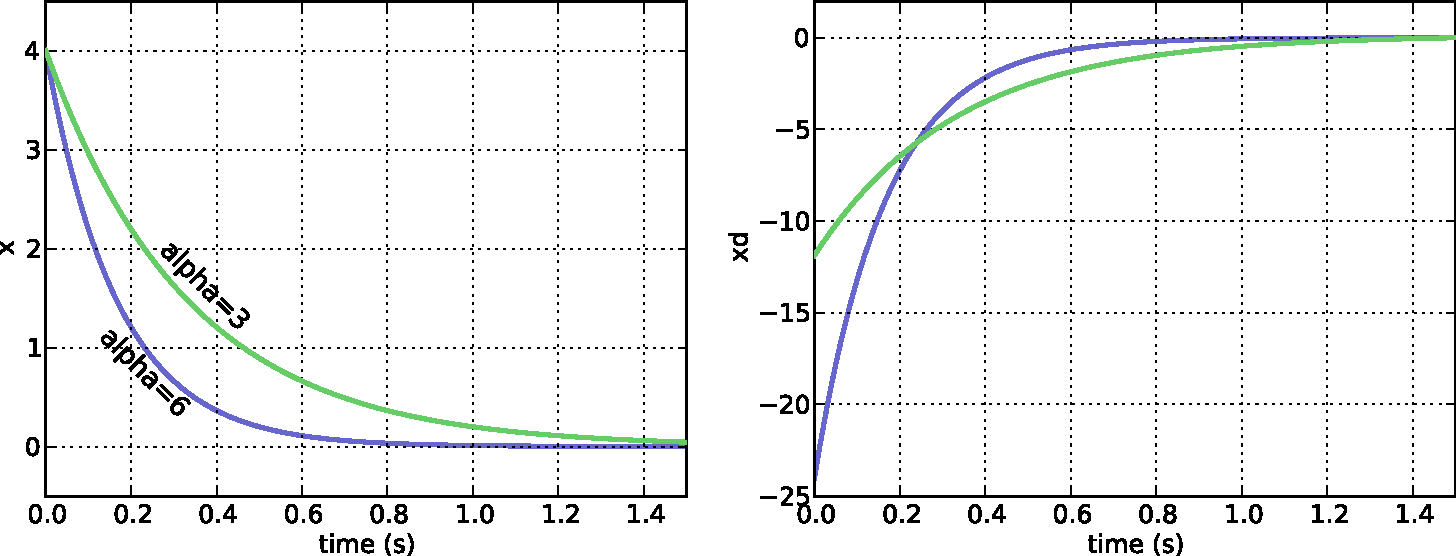
\includegraphics[height=4cm]{exponential_decay-svg}
\caption{Evolution of the exponential dynamical system.}
\end{DoxyImage}


The evolution of many dynamical systems can also be determined analytically, by explicitly solving the differential equation. For instance, $N(t) = x_0e^{-\alpha t}$ is the solution to $\dot{x} = -\alpha x$. Why? Let's plug $x(t) = x_0e^{-\alpha t}$ into $\frac{dx}{dt} = -\alpha x$, which leads to $\frac{d}{dt}(x_0e^{-\alpha t}) = -\alpha (x_0e^{-\alpha t})$. Then derive the left side of the equations, which yields $-\alpha(x_0e^{-\alpha t}) = -\alpha (x_0e^{-\alpha t})$. Q\+E\+D. Note that the solution works for arbitrary $x_0$. It should, because the solution should not depend on the initial state.\hypertarget{page_dyn_sys_dynsys_implementation1}{}\subsubsection{Implementation}\label{page_dyn_sys_dynsys_implementation1}
{\itshape  In the object-\/oriented implementation of this module, all dynamical systems inherit from the abstract Dynamical\+System class. The analytical solution of a dynamical system is computed with Dynamical\+System\+::analytical\+Solution, which takes the times {\ttfamily ts} at which the solution should be computed, and returns the evolution of the system as {\ttfamily xs} and {\ttfamily xds}.}

{\itshape A system's differential equation is implement in the function Dynamical\+System\+::differential\+Equation, which takes the current state {\ttfamily x}, and computes the rates of change {\ttfamily xd}. The functions Dynamical\+System\+::integrate\+Start() and Dynamical\+System\+::integrate\+Step() are then used to numerically integrate the system as follows (using the example plotted above)\+:}

{\itshape 
\begin{DoxyCode}
\textcolor{comment}{// Make exponential system that decays from 4 to 0 with decay constant 6, and tau=1.0}
\textcolor{keywordtype}{double} alpha = 6.0;                \textcolor{comment}{// Decay constant}
\textcolor{keywordtype}{double} tau = 1.0;                  \textcolor{comment}{// Time constant }
VectorXd x\_init(1); x\_init << 4.0; \textcolor{comment}{// Initial state (a 1D vector with the value 4.0 inside using Eigen
       comma initializer)}
VectorXd x\_attr(1); x\_attr << 0.0; \textcolor{comment}{// Attractor state}
DynamicalSystem* dyn\_sys = \textcolor{keyword}{new} ExponentialSystem(tau, x\_init, x\_attr, alpha);

Eigen::VectorXd x, xd;
dyn\_sys->integrateStart(x,xd); \textcolor{comment}{// Start the integration}
\textcolor{keywordtype}{double} dt = 0.01;
\textcolor{keywordflow}{for} (\textcolor{keywordtype}{double} t=0.0; t<1.5; t+=dt)
\{
  dyn\_sys->integrateStep(dt,x,x,xd);          \textcolor{comment}{// Takes current state x, integrates system, and writes next
       state in x, xd}
  cout << t << \textcolor{stringliteral}{" "} << x << \textcolor{stringliteral}{" "} << xd << endl; \textcolor{comment}{// Output current time, state and rate of change}
\}
\textcolor{keyword}{delete} dyn\_sys;
\end{DoxyCode}
}

{\itshape {\itshape Remark}. Both analytical\+Solution and differential\+Equation functions above are const, i.\+e. they do not change the Dynamical\+System itself.}

{\itshape {\itshape Remark}. Dynamical\+System\+::integrate\+Step uses either Euler integration, or 4-\/th order Runge-\/\+Kutta. The latter is more accurate, but requires 4 calls of Dynamical\+System\+::differential\+Equation() instead of 1). Which one is used can be set with Dynamical\+System\+::set\+\_\+integration\+\_\+method(). To numerically integrate a dynamical system, one must carefully choose the integration time dt. Choosing it too low leads to inaccurate integration, and the numerical integration will diverge from the 'true' solution acquired through analytical solution. See \href{http://en.wikipedia.org/wiki/Euler%27s_method}{\tt http\+://en.\+wikipedia.\+org/wiki/\+Euler\%27s\+\_\+method} for examples. Choosing dt depends entirely on the time-\/scale (seconds vs. years) and parameters of the dynamical system (time constant, decay parameters).}

{\itshape }\hypertarget{page_dyn_sys_dynsys_implementation1_plotting}{}\subsubsection{Plotting}\label{page_dyn_sys_dynsys_implementation1_plotting}
{\itshape  If you save the output of a dynamical in a file with format (where D is the dimensionality of the system, and T is the number of time steps) \begin{DoxyVerb}x^0_0 x^1_0 .. x^D_0   xd^0_0 xd^1_0 .. xd^D_0   t_0   
x^0_1 x^1_1 .. x^D_1   xd^0_1 xd^1_1 .. xd^D_1   t_1   
   :     :       :         :      :       :       :    
x^0_T x^1_T .. x^D_T   xd^0_T xd^1_T .. xd^D_T   t_T   
\end{DoxyVerb}
 you can plot this output with 
\begin{DoxyCode}
python dynamicalsystems/plotting/plotDynamicalSystem.py file.txt
\end{DoxyCode}
}

{\itshape }\hypertarget{page_dyn_sys_dynsys_implementation1_demo}{}\subsubsection{Demos}\label{page_dyn_sys_dynsys_implementation1_demo}
{\itshape  A demonstration of how to initialize and integrate an Exponential\+System is in \hyperlink{demoExponentialSystem_8cpp}{demo\+Exponential\+System.\+cpp}}

{\itshape A more complete demonstration including all implemented dynamical systems is in \hyperlink{demoDynamicalSystems_8cpp}{demo\+Dynamical\+Systems.\+cpp}. If you call the resulting executable with a directory argument, e.\+g. 
\begin{DoxyCode}
./demoDynamicalSystems /tmp/demoDynamicalSystems
\end{DoxyCode}
 it will save results to file, which you can plot with for instance\+: 
\begin{DoxyCode}
python plotDynamicalSystem.py /tmp/demoDynamicalSystems/ExponentialSystem/results\_rungekutta.txt
python plotDynamicalSystem.py /tmp/demoDynamicalSystems/ExponentialSystem/results\_euler.txt
\end{DoxyCode}
 Different test can be performed with the dynamical system. The test can be chosen by passing further argument, e.\+g. 
\begin{DoxyCode}
./demoDynamicalSystems /tmp/demoDynamicalSystems rungekutta euler
\end{DoxyCode}
 will integrate the dynamical systems with both the Runge-\/\+Kutta and simple Euler method. The available tests are\+: \begin{DoxyItemize}
\item \char`\"{}rungekutta\char`\"{} -\/ Use 4th-\/order Runge-\/\+Kutta integration (more accurate, but more calls of Dynamical\+System\+::differential\+Equation) \item \char`\"{}euler\char`\"{} -\/ Use simple Euler integration (less accurate, but faster) \item \char`\"{}analytical\char`\"{} -\/ Use the analytical solution instead of numerical integration \item \char`\"{}tau\char`\"{} -\/ Change tau before doing numerical integration \item \char`\"{}attractor\char`\"{} -\/ Change the attractor state during numerical integration \item \char`\"{}perturb\char`\"{} -\/ Perturb the state during numerical integration\end{DoxyItemize}
To compare for instance the analytical solution with the Runge-\/\+Kutta integration in a plot, you can do 
\begin{DoxyCode}
python plotDynamicalSystemComparison.py /tmp/demoDynamicalSystems/ExponentialSystem/results\_analytical.txt 
       /tmp/demoDynamicalSystems/ExponentialSystem/results\_rungekutta.txt
\end{DoxyCode}
}

{\itshape }\hypertarget{page_dyn_sys_sec_dyn_sys_properties}{}\subsection{Properties and Features of Linear Dynamical Systems}\label{page_dyn_sys_sec_dyn_sys_properties}
\hypertarget{page_dyn_sys_sec_dyn_sys_convergence}{}\subsubsection{Convergence towards the Attractor}\label{page_dyn_sys_sec_dyn_sys_convergence}
In the limit of time, the dynamical system for exponential decay will converge to 0 (i.\+e. $x(\infty) = x_0e^{-\alpha\infty} = 0$). The value 0 is known as the {\itshape attractor} of the system. For simple dynamical systems, it is possible to {\itshape proove} that they will converge towards the attractor.

Suppose that the attractor state in our running example is not 0, but 1. In that case, we change the attractor state of the exponential decay to $x^g$ ( $g$=goal) and define the following differential equation\+: \begin{eqnarray*} \dot{x} =& -\alpha(x-x^g) & \mbox{~with attractor } x^g \end{eqnarray*}

This system will now converge to the attractor state $x^g$, rather than 0.


\begin{DoxyImage}
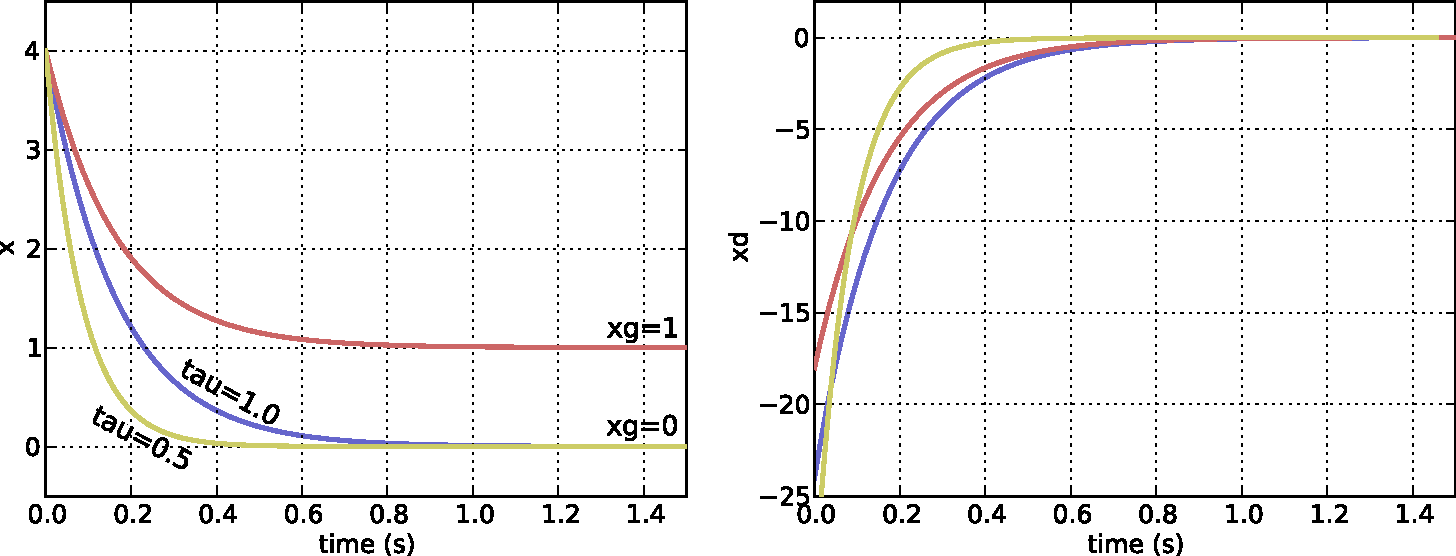
\includegraphics[height=4cm]{change_tau_attr-svg}
\caption{Changing the attractor state or time constant.}
\end{DoxyImage}
\hypertarget{page_dyn_sys_sec_dyn_sys_perturbations}{}\subsubsection{Robustness to Perturbations}\label{page_dyn_sys_sec_dyn_sys_perturbations}
Another nice feature of dynamical systems is their robustness to perturbations, which means that they will converge towards the attractor even if they are perturbed. The figure below shows how the perturbed system (cyan) converges towards the attractor state just as the unperturbed system (blue) does.


\begin{DoxyImage}
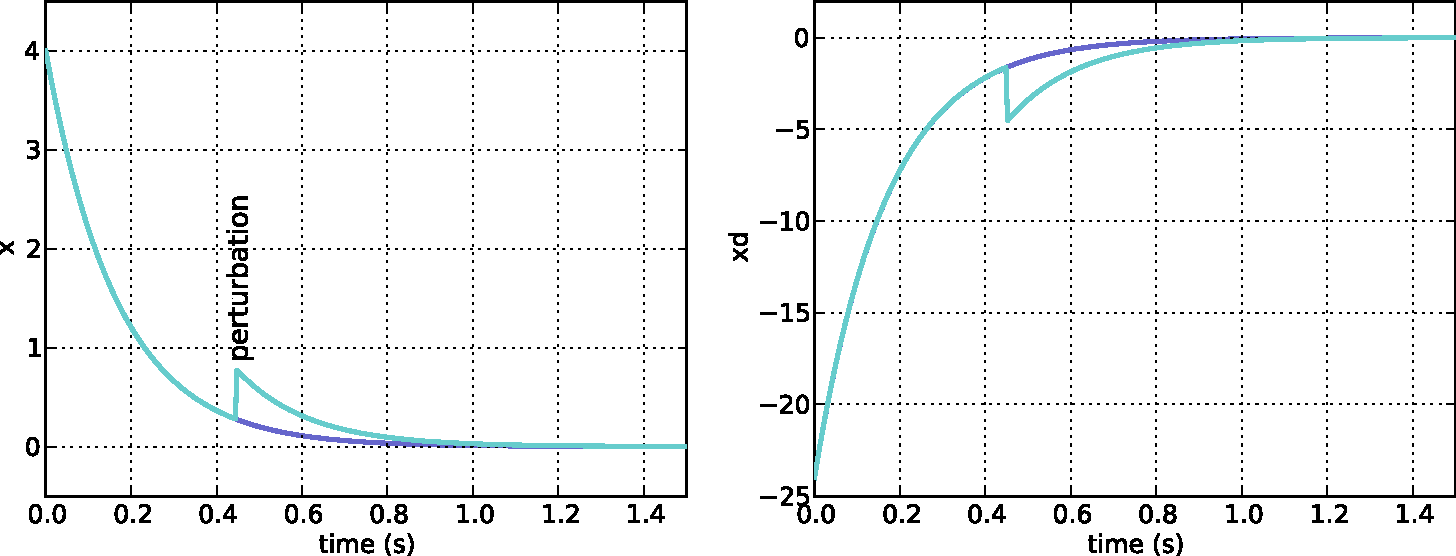
\includegraphics[height=4cm]{perturb-svg}
\caption{Perturbing the dynamical system.}
\end{DoxyImage}
\hypertarget{page_dyn_sys_sec_dyn_sys_time_constant}{}\subsubsection{Changing the speed of convergence\+: The time constant}\label{page_dyn_sys_sec_dyn_sys_time_constant}
The rates of change computed by the differential equation can be increased or decreased (leading to a faster or slower convergence) with a {\itshape time} {\itshape constant}, which is usually written as follows\+:

\begin{eqnarray*} \tau\dot{x} =& -\alpha(x-x^g)\\ \dot{x} =& (-\alpha(x-x^g))/\tau \end{eqnarray*}

{\itshape Remark}. For an exponential system, decreasing the time constant $\tau$ has the same effect as increasing $\alpha$. For more complex dynamical systems with several parameters, it is useful to have a separate parameter that changes only the speed of convergence, whilst leaving the other parameters the same.\hypertarget{page_dyn_sys_sec_dyn_sys_multi}{}\subsubsection{Multi-\/dimensional states}\label{page_dyn_sys_sec_dyn_sys_multi}
The state $x$ need not be a scalar, but may be a vector. This then represents a multi-\/dimensional state, i.\+e. $\tau\dot{\mathbf{x}} = -\alpha(\mathbf{x}-\mathbf{x}^g)$. In the code, the size of the state vector $dim(\mathbf{x})\equiv dim(\dot{\mathbf{x}})$ of a dynamical system is returned by the function Dynamical\+System\+::dim()\hypertarget{page_dyn_sys_sec_dyn_sys_autonomy}{}\subsubsection{Autonomy}\label{page_dyn_sys_sec_dyn_sys_autonomy}
Dynamical system that do not depend on time are called {\itshape autonomous}. For instance, the formula $ \dot{x} = -\alpha x$ does not depend on time, which means the exponential system is autonomous.\hypertarget{page_dyn_sys_Implementation}{}\subsubsection{Implementation}\label{page_dyn_sys_Implementation}
{\itshape  The attractor state and time constant of a dynamical system are usually passed to the constructor. They can be changed afterwards with with Dynamical\+System\+::set\+\_\+attractor\+\_\+state and Dynamical\+System\+::set\+\_\+tau. Before integration starts, the initial state can be set with Dynamical\+System\+::set\+\_\+initial\+\_\+state. This influences the output of Dynamical\+System\+::integrate\+Start, but not Dynamical\+System\+::integrate\+Step.}

{\itshape Further (first order) linear dynamical systems that are implemented in this module is a Sigmoid\+System (see \href{http://en.wikipedia.org/wiki/Exponential_decay}{\tt http\+://en.\+wikipedia.\+org/wiki/\+Exponential\+\_\+decay} and \href{http://en.wikipedia.org/wiki/Sigmoid_function}{\tt http\+://en.\+wikipedia.\+org/wiki/\+Sigmoid\+\_\+function}), as well as a dynamical system that has a constant velocity (Time\+System), so as to mimic the passing of time (time moves at a constant rate per time ;-\/)}

{\itshape  \begin{eqnarray*} \dot{x} =& -\alpha (x-x^g) & \mbox{exponential decay/growth} \label{equ_}\\ \dot{x} =& \alpha x (\beta-x) & \mbox{sigmoid} \label{equ_}\\ \dot{x} =& 1/\tau & \mbox{constant velocity (mimics the passage of time)} \label{equ_}\\ \end{eqnarray*}}

{\itshape 
\begin{DoxyImage}
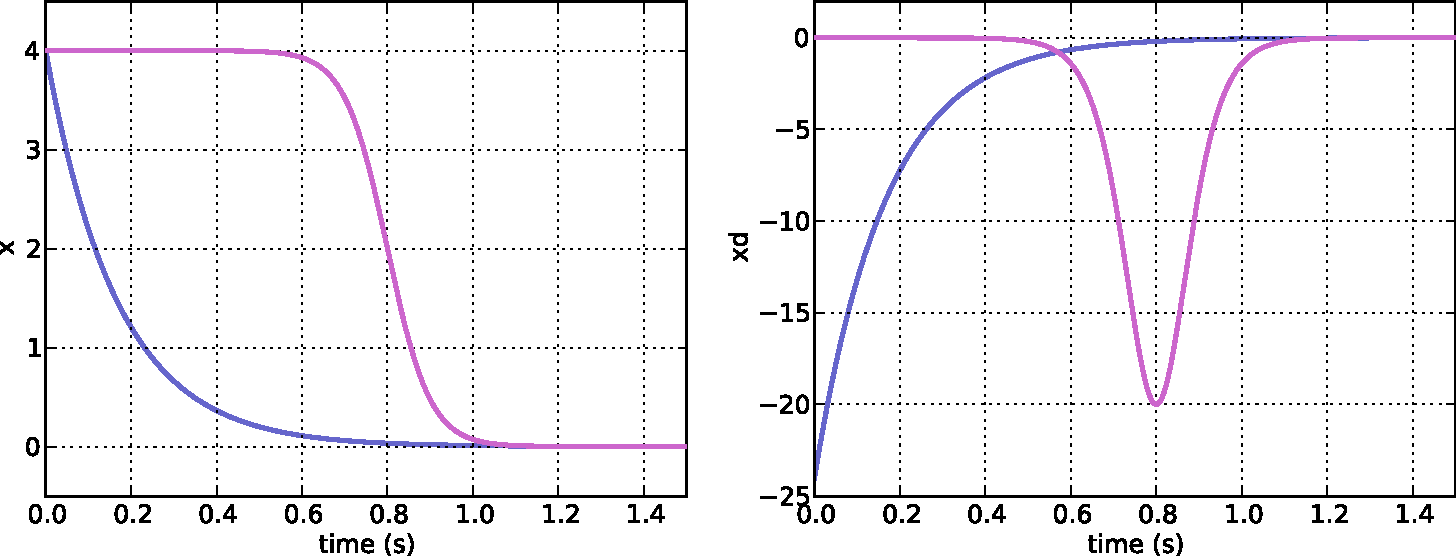
\includegraphics[height=4cm]{sigmoid-svg}
\caption{Exponential (blue) and sigmoid (purple) dynamical systems.}
\end{DoxyImage}
}

{\itshape }\hypertarget{page_dyn_sys_dyn_sys_second_order_systems}{}\subsection{Second-\/\+Order Systems}\label{page_dyn_sys_dyn_sys_second_order_systems}
The {\bfseries order} of a dynamical system is the order of the highest derivative in the differential equation. For instance, $\dot{x} = -\alpha x$ is of order 1, because the derivative with the highest order ( $\dot{x}$) has order 1. Such a system is known as a first-\/order system. All systems considered so far have been first-\/order systems, because the derivative with the highest order, i.\+e. $ \dot{x} $, has always been of order 1.\hypertarget{page_dyn_sys_dyn_sys_spring_damper}{}\subsubsection{Spring-\/\+Damper Systems}\label{page_dyn_sys_dyn_sys_spring_damper}
An example of a second order system (which also has terms $ \ddot{x} $) is a spring-\/damper system (see \href{http://en.wikipedia.org/wiki/Damped_spring-mass_system}{\tt http\+://en.\+wikipedia.\+org/wiki/\+Damped\+\_\+spring-\/mass\+\_\+system}), where $k$ is the spring constant, $c$ is the damping coefficient, and $m$ is the mass\+:

\begin{eqnarray*} m\ddot{x}=& -kx -c\dot{x} & \mbox{spring-damper (2nd order system)} \label{equ_}\\ \ddot{x}=& (-kx -c\dot{x})/m & \end{eqnarray*}\hypertarget{page_dyn_sys_dyn_sys_critical_damping}{}\subsubsection{Critical Damping}\label{page_dyn_sys_dyn_sys_critical_damping}
A spring-\/damper system is called critically damped when it converges to the attractor as quickly as possible without overshooting, as the red plot in \href{http://en.wikipedia.org/wiki/File:Damping_1.svg}{\tt http\+://en.\+wikipedia.\+org/wiki/\+File\+:\+Damping\+\_\+1.\+svg}. This happens when $c = 2\sqrt{mk}$.\hypertarget{page_dyn_sys_dyn_sys_rewrite_second_first}{}\subsubsection{Rewriting one 2nd Order Systems as two 1st Order Systems}\label{page_dyn_sys_dyn_sys_rewrite_second_first}
For implementation purposes, it is more convenient to work only with 1st order systems. Fortunately, we can expand the state $ x $ into two components $ x = [y~z]^T$ with $ z = \dot{y}$, and rewrite the differential equation as follows\+:

$ \left[ \begin{array}{l} \dot{y} \\ \dot{z} \end{array} \right] = \left[ \begin{array}{l} z \\ (-ky -cz)/m \end{array} \right] $

With this rewrite, the left term contains only first order derivatives, and the right term does not contain any derivatives. This is thus a first order system. Integrating such an expanded system is done just as one would integrate a dynamical system with a multi-\/dimensional state\+:\hypertarget{page_dyn_sys_Implementation}{}\subsubsection{Implementation}\label{page_dyn_sys_Implementation}
{\itshape  The constructor Dynamical\+System\+::\+Dynamical\+System immediately converts second order systems into first order systems with an expanded state.}

{\itshape The function Dynamical\+System\+::dim() returns the size of the entire state vector $ x = [y~z]$, the function Dynamical\+System\+::dim\+\_\+orig() return the size of only the $ y $ component. The attractor and initial state must always have the size returned by Dynamical\+System\+::dim\+\_\+orig(). } 